\begin{figure*}[!ht]
\centerline{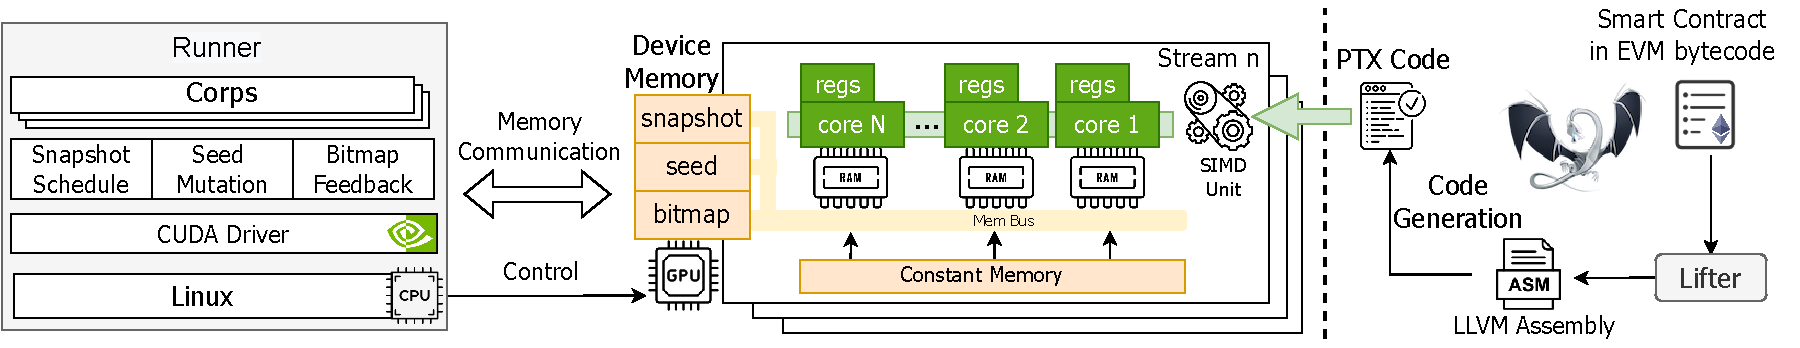
\includegraphics[width=\textwidth]{images/GFL-overview.drawio.pdf}}
\caption{The overview of {\tool}. {\translator} first translates the given bytecode to a PTX code which can be loaded by GPU for parallel fuzzing, under the guidance of {\runner}. {\translator} only executes once for each fuzzing application.}
\vspace{-0.1in}
\label{fig:overview}
\end{figure*}

\section{Design}
\label{sec:design}

Figure~\ref{fig:overview} depicts the architecture of the {\tool}, which tests a smart contract thousands times together using the GPU SIMD architecture.
% Based on binary translation technology, {\tool} can fuzz the smart contract even if its source code is unavailable.
%
To be specific, the process pipeline of {\tool} consists of five steps. 
%
First, given an EVM bytecode, {\translator} translates it into a functional equivalent LLVM assembly, where the opcodes for EVM components (e.g., stack, memory and storage) are abstracted in LLVM memory operations.
% implemented in device functions to avoid CPU.
%
Second, {\translator} rewrites the memory operations of the LLVM assembly from the on-the-fly translation, enabling the fuzzing threads are free of branches via data parallelism.
% Second, {\wrapper} creates a GPU kernel function in LLVM IR to wrap the contract code from {\translator}, for the parallel execution in GPU. The kernel function schedules graphic memory for thousands of GPU threads, allowing all threads to independently execute with different input. The wrapped LLVM assembly will be translated into a PTX executable as the final fuzzing target. 
%
The third step is the code generation producing a PTX smart contract from the established LLVM assembly, using the LLVM backend\cite{llvm2021bin}.
Next, {\runner} generates seeds and executes them with the PTX smart contract in thousands of threads. 
{\runner} is also equipped with snapshots strategies and coverage-based feedback to guide the seed mutation.
At last, {\runner} mutates for more seeds and repeats the fourth step until any bugs are detected. 

This section introduces {\runner} and then {\translator}.
The first part explains the target and challenges in fuzzing a smart contract on GPU.
The second part answers the reasons behind the design choices of {\translator} in generating a smart contract equipped with the components required by {\runner}.


\subsection{{\runner}: High Performance Fuzzing}
Throughput indicates the number of seeds that can be tested by fuzzers in a time unit. The execution speed of the target program is the fundamental factor in fuzzing throughput\cite{fuzzan_atc}. 
%
Unfortunately, existing smart contract fuzzers\cite{confuzzius_eurosp,echidna_issta} suffer from serious throughput bottlenecks, because smart contracts are designed to run on a virtual machine rather than the native environment. 
%
% It contrasts to task parallelism as another form of parallelism.
To improve throughput, they did apply task parallelism to test multiply seeds together, where the target application is executed as several processes in a multi-cores machine.
However, fuzzing smart contracts on a virtual machine will bring too much overhead, because these virtual machines compromise performance for
deterministic execution at runtime.
%
Although one possible solution is to run EVM bytecode as CPU native code via JIT (just-in-time) compilation, the fuzzers will still share the same throughput bottlenecks with the classical fuzzers like AFL\cite{afl} and Angora\cite{angora_sp}. 
For example, the maximum number of parallel fuzzers cannot exceed 128 because of the limited CPU cores.
% Under such execution layout, the existing smart contract fuzzers have to maintain a 
Therefore, in terms of fundamental aspects, the existing fuzzing technologies cannot achieve high throughput in testing smart contracts (See \S~\ref{} for more details).


We believe the key of improving fuzzing throughput is running the smart contract in as many parallel threads as possible without using blockchain virtual machines. 
%
Fuzzing is an ideal workload for parallel execution because all fuzzing threads are naturally free of lock.
To be specific, in each fuzzing thread, we can run the target smart contract independently with its own context, i.e., stack, memory and registers. 
The only synchronization event is used to wait for the end of all fuzzing threads so that the collected coverage information can guide the fuzzer to mutate new seeds.
%
The more threads we can schedule, the higher throughput the fuzzer can achieve.
That is the reason why we choose to fuzz smart contracts on GPU. 
Different from CPU, GPU is full of stream processors, enabling to run thousands of threads in parallel. 
%
As one of the most powerful CPU, AMD Ryzen Threadripper PRO 5995WX (\$6,499) only has 64 cores, while a NVIDIA RTX3090 (\$999) can provide 10,496 CUDA cores\footnote{The prices come from the official vendor websites.}. 
The incredible computation power of GPU is attractive for parallel fuzzing as long as we can translate a smart contracts into a GPU executable, i.e., PTX\cite{ptx2021doc}. 
%
Since GPU is based on SIMD architecture, we need to apply data parallelism rather than task parallelism.


% Running on CPU, {\runner} will launch a GPU device and fuzz the smart contracts with a batch of seeds together. Once the GPU jobs are finished, {\runner} obtains the coverage information to guide the seed generations. 

% In this section, we mainly elaborate the design and reasons of {\runner}, including SIMD execution for parallel fuzzing, snapshot strategy for handing transaction dependency (TBD).
%
% These strategies raise functional requirements to the smart contract and they can explain the design choices of the bytecode translation in \S~\ref{design:translator}.





\subsubsection{Asynchronous Calls for GPUs}

\begin{figure}[t]
\centerline{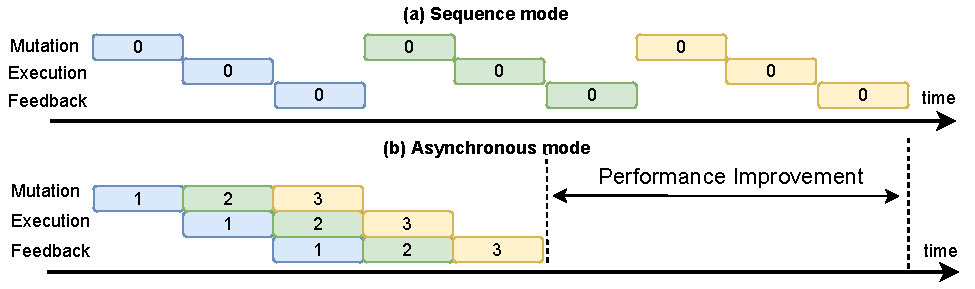
\includegraphics[width=0.5\textwidth]{images/GFL-async_cpy.drawio.pdf}}
\caption{Fuzzing Timelines}
\vspace{-0.1in}
\label{fig:async_cpy}
\end{figure}

GPU can load a PTX code which the SIMD unit dispatches to every GPU core (See Figure~\ref{fig:overview}(c)). 
In each moment, the running cores must execute the same code together but accept different seeds via data parallelism\cite{cuda2006datapara}.
We define $i$ as the thread ID that the thread can use to compute its data from the all threads data.
%
{\runner} creates a data mapping for the input data for each thread, enabling thread $i$ can extract a seed to test.
%
Since GPU and CPU are two independent devices, {\runner} can asynchronously invoke a GPU to execute the smart contract and immediately use the CPU to run the fuzzing tasks such as seed mutation and bitmap feedback.
%
Based on thread ID, we can schedule the GPU threads together with the corresponding fuzzing tasks on a CPU. 

% When branch instructions are dispatched, some threads may execute different paths, resulting they run in serial rather than in parallel. 
%
% That is the reason why SIMD code should reduce branch divergence\cite{branchdiver2011gpgpu} to improve performance.
%

% 需要用i干什么,vectorized smart contract
% 如何利用GPU SIMD
% 进而解释async mode下为何要调整thread id

To this end, we create several CUDA streams.
Each stream consists of three tasks such as seeds mutation, smart contract execution and bitmaps feedback. 
We define $D_i$ as one stream, where each stream consists of $T$ threads. 
The threads in the same stream will be executed in parallel. 
All streams share the same GPU device memory, thus the threads in different streams should compute their global ID to access the expected memory for data parallelism.
%
Since the threads ID in different streams are not continuous but re-increase from zero, we adjust the thread ID to allow each thread to access its memory.
%
When $D_l$ is submitted to a GPU from the CPU end, each thread ID should be increased by an offset.
$$
i = T*l
$$

\noindent\textbf{Compared with Classical Work.}
To the best of our knowledge, existing fuzzers are implemented on CPU. 
Their fuzzing steps are tasks, which are required to be executed in sequence on CPUs.
On the one hand, the target application cannot run until the mutated seeds are prepared. 
On the other hand, fuzzers have to wait the target application execution ends and then can use feedback strategies. 
%
To improve the throughput, {\tool} is designed to reduce the time intervals between fuzzing tasks via asynchronous execution.
%
In Figure~\ref{fig:async_cpy}, we show the timelines for sequence mode (a) and asynchronous mode (b) in a three rounds fuzzing. 
{\tool} creates three stream pipelines to handle the three group of fuzzing tasks in asynchronous mode. 
The jobs in the same stream are highlighted in the same color. 
In the first time slot, we mutate seeds on CPU only. In the next slot, $D_1$ and stream $D_2$ run together, which executes the smart contract on GPU and mutates seeds on CPU, respectively. 
%
At last, {\tool} can finish the fuzzing work within five time slots, which is less than the traditional methodology (nine slots).
%
% Moreover, the asynchronous mode enables {\tool} to reduce the delay of memory latency. \cite{} analyzes the CUDA overhead and finds transferring data between CPU and GPU is time-consuming. {\tool} can invoke another streams when the memory bus of GPU is stuck to one stream job. 



\begin{figure}[ht]
    \centering
    \lstinputlisting[language=Solidity,linewidth={\linewidth},frame=tb,basicstyle=\footnotesize\ttfamily]{code/tx_dep.sol}
    \vspace{-0.1in}
    \caption{An Example for Transaction Dependency.}
    \label{fig:code_tx_dep}
\end{figure}

\subsubsection{Snapshot Schedule}
\label{design:snapshot}
Smart contract is a stateful program, which maintains state variables in its storage, i.e., a key-value mapping. Since state variables can be a part of branch conditions, some branches can only be explored when the smart contract storage is set to specific content. 
We call it transaction dependency.
%
Figure~\ref{fig:code_tx_dep} shows an example, where the integer overflow bug in function $vul()$ can only be triggered when the state variable named $key$ is set to \texttt{false} via executing $unlock()$ first. 
%
To explore more branches, existing fuzzers generate a transactions sequence as the seed to handle the transaction dependency\cite{confuzzius_eurosp, echidna_issta, ilf_ccs}. 
%
To be specific, they first choose one transaction and then combined it with other transactions to generate a sequence-based seed. 
However, they may execute duplicated transactions. 
The redundant execution wastes computational resources, resulting in low throughput. 
%
To address this issue, we design storage snapshots to switch fuzzing states. 
An interesting seed can explore new branches of the smart contract. We test the interesting seed and call the finalized content of the storage as an interesting state.
%
Hence, each snapshot is a byte string representing the storage content. 
%
In the next fuzzing iteration, {\tool} can reload a storage snapshot to further test the smart contract, i.e., the storage updated by $vul()$ in Figure~\ref{fig:code_tx_dep}.
%
By switching snapshots, {\tool} can allocate more energy on the interesting state to facilitate the transaction dependency without executing duplicated transactions. Moreover, we can use on-chain data as the storage snapshot to test real-world smart contracts.

Since storage snapshot switches require additional data exchange between CPU and GPU, we should reduce the overhead due to the memory latency between CPU and GPU, which is the main bottleneck in CUDA programming\cite{}. 
To this end, we further design Redirect-On-Write (ROW) storage snapshot.
%
The data originally associated with the master volume remains in place; the new data is written to a snapshot\cite{row2021ibm}.
%
This design is based on our observation that one transaction usually only modify a few storage variables. 
Therefore, a smart contract in different stages may share a part of the same storage content.
%
Here are some details.
Before launching the GPU threads, we load a storage snapshot as the master volume, denoted as $m$, which is an read-only array exposing to all threads.
$N$ is a snapshot vector representing every thread snapshot, where $N_i$ indicates the ROW snapshot of the storage used by thread $i$.
%
If thread $i$ executed an interesting seed, we combine $N_i$ with $m$ as a full volume. 
In the next fuzzing round, {\runner} can select this combined storage as a new master volume.



\subsubsection{Coverage Feedback}
\label{sec:runner:coverage}
{\runner} records the coverage information to a bitnap.
Bitmap is a serial array, where the compile-time inserted instructions will update the bitmap when the smart contract is running. 
%
The bitmap content should contain both the touched edges and changes of the state variable to guide the stateful fuzzing.


Traditional coverage-based fuzzers feedback seed mutation based on the explored branches.
For example, AFL uses a tuple $(src, dst)$ to record a touched edge, i.e., a control flow from one basic block to another one. Whenever a basic block is executed, the bitmap byte in the index of $src \ll 1 \oplus dst$ increases by one. 
Since smart contracts are stateful, we extend the bitmap to reflect the changes of the state variables. 
To be specific, the index of each explored edge in bitmap is set to $state_0 \oplus ... \oplus state_n \oplus src \ll 1 \oplus dst$, where $state_i$ indicates one storage variable. (TBD)


Each thread should record its coverage information in its own bitmap, which will cost too much memory. 
To reduce memory consumption, we use a temporary memory as the bitmap and encode the coverage from all existing bitmaps to an array named \texttt{virgin\_bits}\cite{afl}, denoted as $b$. 
\texttt{virgin\_bits} has the same size from a bitmap.
Each byte (i.e., $b_j$) represents whether the corresponding branch is touched or not.
Initially, the entire \texttt{virgin\_bits} is fully masked, i.e., each byte value is 0xff.
We set $b_j$ to zero if there exist one bitmap touching the branch $j = hash(src,dst,states)$. 
If $b_j$ remains 0xff, {\runner} considers the branch have not yet touched by any seeds. 

\subsubsection{Seeds Mutation}
\label{design:mutation}
If a seed is interesting, {\runner} will mutate it to generate more seeds. 
Each seed is a byte array, consisting three parts such as \texttt{calldata}, \texttt{calldatasize} and \texttt{callvalue}, representing the input of smart contract, the size of \texttt{calldata} and the amount of cryptocurrency (i.e., Ether), respectvely.  
%
The first fourth bytes of \texttt{calldata} represent a function signature, and its following bytes are its function arguments serialized based on the ABI.
ABI (Application Binary Interface) is a Json-format file describing the headers of the smart contract functions, such as signatures and arguments types. 
Thanks to the parallel fuzzing, {\runner} is able to test all functions with thousands of threads. 
In the beginning, we establish the fourth bytes of each seed as one function signature and then generate initial bytes as the function arguments.
During the fuzzing, {\runner} focuses on mutating the arguments bytes based on the ABI.
The sequence of bytes belong to the same function argument should be mutated together.
%
% In \S~\ref{}, we have leveraged snapshot mechanism to select the tested function of a smart contract. 
%
% In this part, we focus on mutating the function arguments. Specifically, we mutate the calldata starting from the fourth byte. 
%
% As calldata is constructed following the ABI grammar, some sequence of bytes belong to the same function argument. Thus, they should be mutated together.
%
% To this end, we parse the ABI and then identify the affine types between the raw calldata bytes and high-level function arguments. 
%
According to the function headers recorded in ABI, we mutate the bytes according to the types of the function arguments. 
For each byte sequence we mutate them using AFL\cite{afl} approaches such as bit flipping, bytes walking and so on.
Note that, we update \texttt{calldatasize} for the new seed. \texttt{callvalue} is set to a large constant, assuming we have enough cryptocurrency. 

Apart from seeds, {\runner} also provides some misc for the testing smart contract, such as  \texttt{tx.sender} and \texttt{tx.origin}, representing the account address of the transaction sender and the original sender, respectively. 
We assume {\tool} has the owner privilege to test the smart contract, thus both \texttt{msg.caller} and \texttt{tx.origin} are set to pre-defined constants.
    

\subsection{{\translator}: Smart Contract Generation}
\label{design:translator}
We rewrite the target smart contracts in IR for various purposes, such as 1) functional equivalent translation, 2) compile-time instrumentation for the bitmap and sanitizers 3) changing to vectorized operations.
%
The output of {\translator} is an LLVM assembly, which can be generated into a PTX code.
%
% Broadly speaking, there are two approaches to obtain the llvm assembly of an Ethereum smart contract: 1) Source code compilation by converting Solidity to C++ first and generate IR from clang\cite{}; 2) Binary translation from an EVM bytecode. 
% We choose to use binary translation because blockchain public every smart contract and encourage nodes to execute and verify them, for satisfying consensus protocol. {\tool} can test the real-world smart contract as it is deployed. 
% We exclude the source code approach because Solidity does not support LLVM and the existing Solidity to C++ parser has serious compatibility issues as Solidity grammar updates quite often. Moreover, even there exist available source code tools, developers have to recompile the target with flags, which may be opaque for the testing. 

\subsubsection{SIMD Smart Contract}
To enable a smart contract run in SIMD mode, the PTX smart contract should be a vectorized code\cite{nuzman2011vapor}. 
%
We create a sequence of bytes in the GPU memory to maintain the seeds vector for all fuzzing threads, denoted as $S$.  
$S_{i,j}$ indicates the $j$ byte of the seed used by the thread $i$.  
Each seed is padded to a fix size for threads to access it with a runtime offset.
Since the PTX smart contract uses memory operations to represent the EVM opcodes on EVM memory and EVM stack, we allocate a data vector for each EVM component such as stack and memory in every thread, denoted as $\mu_i$ and $\nu_i$, respectively. 
Therefore, each individual thread obtain its seed $S_i$ and run its SIMD code to update the expected device memory such as $\mu_i$ and $\nu_i$. For fuzzing, we also reload the storage snapshot $N_i \cup m$ and record the coverage information in the bitmap $B_{i\%32}$. The final output of the threads is the \texttt{virgin\_bits}:
$$
I \times (N_i \cup m) \times S_i \times (\mu_i, \nu_i) \times B_{i\%32}= b
$$
, where $I$ is the SIMD code shared by all threads. 
Note that, we ignore the output of EVM smart contract because it contributes nothing to bug detection.
% To execute threads in SIMD scheme, we create a piece of device memory for each threads to run, such as loading a seed, stack operations, accessing memory and updating the coverage bitmap. 
% To be specific, the input data and output region is equally divided, and each portion is distributed to a specific thread according to its auto-increment ID (i.e., thread ID). 
%
% ------ an example of data layout ----------
% threadIdx = grid.x * block.x * thread.idx

% transaction size: why not use compact mode. 
% Our memory model is strided
% https://developer.nvidia.com/blog/how-access-global-memory-efficiently-cuda-c-kernels/
% aligned memory.
% -------------------------------------------

\subsubsection{Opcode Lifting}
To rewrite the bytecode more flexible and precise, we build an IR-based framework using LLVM intermediate representation\cite{lattner2004llvm}.

\noindent\textbf{Abstract Stack.}
EVM bytecode is a sequential of stack-based opcodes, which can be lifted to an registers-based LLVM assembly. 
We allocate an LLVM array as the EVM stack (i.e., $\mu_i$) and thus EVM opcodes can be represented as memory operations.
$p_i$ is an LLVM variable maintaining the stack depth of the abstract stack used in the thread $i$.
For example, EVM can push a byte from its stack by executing the opcode named \code{PUSH1 im}, which can be lifted to $\mu_{ip} \gets \code{im}; p \gets p+1$, where $\mu_{ip}$ is the element in the $p$ depth of the abstract stack $\mu_i$, within the thread $i$.


\noindent\textbf{Abstract Memory.}
EVM memory opcodes, i.e., \code{MLOAD}, \code{MSTORE8} and \code{MSTORE8} are lifted to the operations on LLVM memory. 
Thus, each thread can access its abstract memory $\nu_i$.
Since EVM is a big-endian machine, we have to swap the operands of EVM memory opcodes, for running in the little-endian GPU.
For example, the most significant byte will exchange with the 
least significant byte.

\begin{figure}[t]
\begin{algorithm}[H]
\caption{Storing a storage state into the ROW snapshot.}
\label{algo:row_sstore}
\begin{algorithmic}[1]
    \Require $key$, the storage index; $val$, the storage state
    \State $Src \gets initial storage states$
    \State $Snap \gets the storage states snapshot$
    \If{$key \in \{s.key \mid s \in Snap\}$} 
        \State $Snap[key].val = val$
        \State \Return
    \EndIf
\end{algorithmic}
\end{algorithm}
\end{figure}

\noindent\textbf{Abstract Storage.}
Apart from stack and memory, EVM can also store data in a key-value mapping. 
\code{SSTORE} and \code{SLOAD} are two storage opcodes for writing and reading EVM storage, respectively.
To enable {\tool} to handle transaction dependency by switching storage snapshots, we rewrite \code{SSTORE} and \code{SLOAD} to vector operations. Each thread should access its own storage in ROW mode:
%
\begin{itemize}
    \item \code{SSTORE x, y} stores \code{y} to the storage taking \code{x} as the hash key. To handle it, we redirect the written data to the storage snapshot $N_i$, i.e., $N_{i} \gets N_{i} \cup \{x:y\}$.
    
    \item \code{y = SLOAD x} loads \code{y} from the storage taking \code{x} as the hash key. To handle it, we first enquiry $y$ from $N_i$. If $N_i$ does not store for $x$ before, we get $y$ from from $m$. Otherwise, we return zero eventually following the EVM design.
\end{itemize}

\noindent\textbf{Jumps Recovery.}
EVM jump opcodes, i.e., \code{\%JUMP} and \code{\%JUMPI} take a jump destination from the EVM stack. 
To recover the control flow, we lift EVM jumps as table jumps. 
The jump table contains all entries of the basic block disassembled at static.
Therefore, a table jump decides its destination until the GPU runtime when it loads the stack top from the abstract stack.


\noindent\textbf{Environment Opcodes.}
Environment opcodes are a set of EVM opcodes to interact with blockchain environment\cite{evm2021opcodes}.
For example, \code{TIMESTAMP} can obtain the timestamp, and \code{NUMBER} can get the current blockchain height. 
%
Although blockchain clients on CPU-end have provided restful APIs for environment opcodes, it will sharply decrease {\tool} throughput if GPU threads choose to wait the API responses from CPU.
% that we can import to lift the environment opcodes,
%
To run the smart contract in GPU, we need to simulate the environment opcodes inside GPU only.
For example, we run the Keccak256\cite{bertoni2013keccak} hash function inside GPU, representing the EVM smart contract computing a hash via the opcode named \code{SHA3}.
% \begin{itemize}
%     \item `get' approaches: return constants
%     \item hash function: implement the keccak256  method;
%     \item storage accesses: read and store data from a ROW snapshot (See \S~\ref{});
%     \item load input data: load data from the CPU in little endianness.
%     \item memory operations: read and store data from \code{\%mem} in little endianness.
% \end{itemize}
% Note that, each thread only access the local memory to avoid threads synchronization.


% ---------------- storage ---------------------
% Given an initial storage, we schedule thousands GPU threads to test the state. We store the initial storage in global memory as the master volume, broadcasting its content to every thread. Every thread creates a ROW snapshot in its local memory to avoid synchronization. If the seed is interesting, we export the storage snapshot to CPU and combine it with the master volume to build a full storage snapshot.   
% %
% We first initiate a master volume as the initial storage of the smart contract, and then create a Redirect-on-write (ROW) snapshot for each fuzzing thread. The snapshot maintains all storage states of the given smart contract, enabling each GPU thread to use minor memory to record the states changes. 



\subsubsection{Bitmap Vector}
\label{sec:translator:bitmap}

The bitmap should be a vector, enabling GPU threads to update their bitmap together.
Each GPU thread should update its bitmap independently to avoid data racing. One trivial attempt is creating a bitmap for each individual thread, but no GPU can provide so much device memory.
Especially, {\tool} is designed to run tremendous number of threads together, requiring us to schedule GPU memory more efficiently. 
Our solution is reusing the bitmap.
CUDA GPUs always run a warp of threads together (usually in size of 32) and run another warp when the current warp threads are all completed and acknowledged\cite{nvidia2021cuda}. Since the hardware must synchronize all threads in the same warp, we can only allocate 32 bitmaps for the entire GPU launch. 
We denote $B_{ij}$ as the $j$ byte of the bitmap of the thread $i$.
When the warp is synchronized, we label a seed of thread $i$ is interesting whenever its corresponding bitmap ($B_i$) contains new bits. Next, we clear the 32 bitmaps and schedule another 32 threads to reuse them.
%


As aforementioned in \S~\ref{sec:runner:coverage}, we encode all bitmaps into a single \texttt{virgin\_bits}. 
However, in SIMD GPU, we cannot update \texttt{virgin\_bits} by selecting bitmaps one by one due to the data racing. 
For example, thread $i$ may finished later than thread $i+1$, resulting the bitmap records from $B_{i+1}$ is overwritten by $B_i$.
%
To solve this problem, we must update all bytes of \texttt{virgin\_bits} together.
We equally split \texttt{virgin\_bits} and each bitmap into 32 portions and distribute to the 32 warp threads to run together. 
Each portion has $\epsilon = \frac{\texttt{MAP\_SIZE}}{32}$ bytes, where \texttt{MAP\_SIZE} is the bitmap size. 
The warp thread $i$ updates the portion of \texttt{virgin\_bits} starting from $\delta = \epsilon * i$ byte. 
Therefore, each thread should update the $\epsilon$ bytes, denoted as $b_{j}, \delta < j < \delta + \epsilon$.
$b_j$ is computed with the corresponding byte of the 32 bitmaps. 
The formal description is shown below.
$$
\begin{aligned}
b_j &\gets b_j \& \neg B_{kj}, 0 < k < 32
\end{aligned}
$$


\subsubsection{Sanitizers}
Sanitizers are piece of code running with the smart contract to detect bugs at runtime. 
Since one GPU thread crash will terminate all running threads, the sanitizers cannot raise exception like classical work in CPU-end. 
%
We create a signal for each threads, denoted as $\sigma_i$. 
%
Whenever a bug is detected, the smart contract thread will stop to label $\sigma_i$ then finish its execution. 
Based on the content of $\sigma_i$, {\runner} can know what kind of bug is detected and output an report. 